\documentclass[final, usenames, dvipsnames]{beamer}
\mode<presentation>{\usetheme{GWU}}
\usepackage{poster_packages}

\usepackage[orientation=landscape, scale=1.24,debug]{beamerposter} 
%\beamertemplategridbackground[0.1in] % grid for aligning stuff

%\setlength{\abovecaptionskip}{0.1cm}
%\setlength{\belowcaptionskip}{-0.3cm}

\def\newblock{} % Avoid the "\newblock undefined" error. See http://newsgroups.derkeiler.com/Archive/Comp/comp.text.tex/2008-07/msg00381.html"

%-----------------------------------------------------------
\newlength{\colsep}
\newlength{\onecolwidth}
\newlength{\twocolwidth}

\setlength{\paperwidth}{121.92cm} % 48in
\setlength{\paperheight}{91.44cm} % 36in


%\setlength{\onecolwidth}{0.23\textwidth} % Width of one column
%\setlength{\twocolwidth}{0.49\textwidth} % Width of two columns
\setlength{\onecolwidth}{28cm} % Width of one column
\setlength{\twocolwidth}{56cm} % Width of two columns
\newlength{\columnheight}
\setlength{\columnheight}{76.5cm}

\setbeamersize{text margin left=1.5cm,text margin right=0.5cm}

\listfiles

%-----------------------------
% MACROS
%-----------------------------
\def\Emph{\textcolor{RoyalBlue}}
%%%%%%%%%%%%%%%%%%%%%%%%%%%%%%%%%%%%%%%%%%%%%%%%%%%%%%%%%%%%%%%%%%%%%%%%%%%%%%%%%%%%%%
%	TITLE
%%%%%%%%%%%%%%%%%%%%%%%%%%%%%%%%%%%%%%%%%%%%%%%%%%%%%%%%%%%%%%%%%%%%%%%%%%%%%%%%%%%%%%%
\title{\Large Geometric Adaptive Control of Attitude Dynamics on \( \SO \) with State Inequality Constraints}
\author{\Large \textcolor{white}{Shankar Kulumani and Christopher Poole}}
\institute{\large Flight Dynamics and Controls Laboratory (Dr. Taeyoung Lee)\\Department of Mechanical and Aerospace Engineering, School of Engineering and Applied Science}

%----------------------------------------------------------------------------------------

\begin{document}
\begin{frame}[t] % enclose entire poster in a frame
\begin{columns}[T,onlytextwidth] % start of all columns in poster

%-----------------------------------------------------------------------------------------
% FIRST (LEFT) COLUMN
%---------------------------------------------------------------------------------------
\begin{column}{\onecolwidth} % first column start

\begin{block}{Background and Motivation} % Background block
	\begin{itemize}
		\item Autonomous control of vehicles is critical for missions
		\begin{itemize}
			\item Typical operations require extensive planning and human interaction
			\item Vehicles must operate safely in hazardous environments
			\item Applicable to under-water, aerial, and spacecraft scenarios
		\end{itemize}
		\item Key technology for autonomy is large angle reorientations in the presence obstacles
			\begin{itemize}
				\item Spacecraft have sensitive payloads e.g. optical sensors
				\item Reorient while not pointing in dangerous directions e.g. Sun, Moon
			\end{itemize}
	\end{itemize}
	\vspace{0.2in}
	\begin{figure}
        \begin{subfigure}[b]{0.4\columnwidth}%
                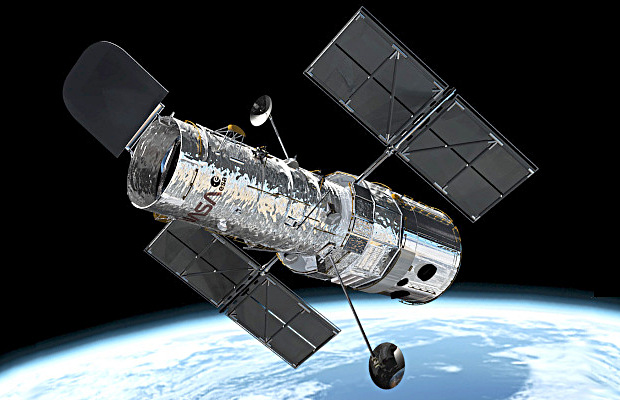
\includegraphics[height=8.5cm]{hubble}%
                \caption*{Hubble}%
                \label{fig:hubble}%
        \end{subfigure}%
        \hfill%
        \begin{subfigure}[b]{0.4\columnwidth}%
                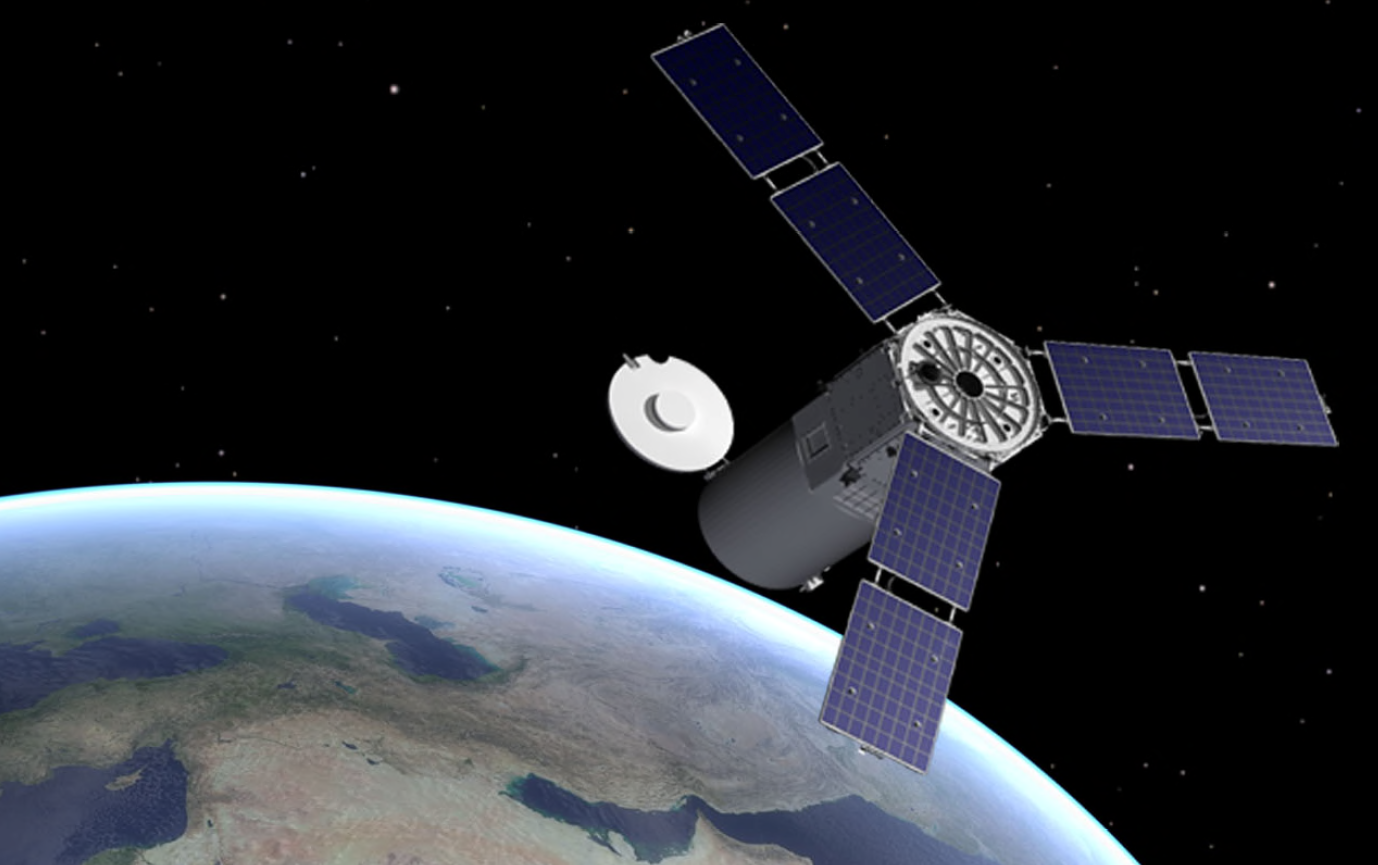
\includegraphics[height=8.5cm]{ors-1}%
                \caption*{Agile S/C}%
                \label{fig:ors}%
        \end{subfigure}%
        \hfill%
		\label{fig:intro}
	\end{figure}
	\vspace{0.2in}
	\begin{itemize}
		\item Problem: reorient a vehicle while avoiding certain directions
		\begin{itemize}
			\item Sensor exclusion zone around the Sun
			\item UAVs manuevering in restricted and congested locations
			\item Laser emitters on industrial robots
		\end{itemize}
	\end{itemize}
\end{block} % end of background block

\begin{block}{Spacecraft Orientation}
	\begin{itemize}
		\item \Emph{Rigid body attitude dynamics} is extensively studied
		\item Configuration manifold is curved and nonlinear
			\begin{itemize}
				\item Dynamics evolve on the Special Orthogonal Group: \( \SO \)
				\item Unique properties: cannot be represented as a linear vector space
			\end{itemize}
		\item Previous work is based on reduced attitude representations
			\begin{itemize}
				\item Euler angles: 24 possible combinations which suffer singularities
				\item Quaternions: no singularities but double cover \( \SO \)
			\end{itemize}
		\item \Emph{Geometric control}: the development of control systems for systems evolving on nonlinear manifolds
			\begin{itemize}
				\item Many systems cannot be defined correctly on Euclidean spaces
				\item Innovative techniques avoid ambiguities and local coordinates and exactly describe the evolution of the system
			\end{itemize}
		
	\end{itemize}
\end{block} 

\begin{block}{Attitude Dynamics} % dynamics block
	\begin{itemize}
		\item Spacecraft is modeled as a rigid body rotating about its center of mass described by the Special Orthogonal Group
			\begin{align*}
				\SO = \braces{R \in \R^{3\times3} \, | \, R^TR = I, \det{R} = 1}
			\end{align*}
		\item \Emph{Euler's equations} of motion govern the dynamics of a rigid body
			\begin{gather*}
				J\dot\Omega + \Omega\times J\Omega = u+W(R,\Omega)\Delta ,\label{eqn:Wdot}\\
				\dot R = R\hat\Omega ,\label{eqn:Rdot}
			\end{gather*}
		\item \( R \in \SO \) defines the orientation of the spacecraft with respect to an inertial reference frame
		\item \( W(R, \Omega) \Delta \) models a wide range of external disturbances
		\begin{itemize}
			\item Solar radiation pressure (SRP)
			\item Gravity gradient moment
			\item Air turbulence and gusts
			\item Unknown mass distribution 
		\end{itemize}
	\end{itemize}
	
\end{block} % end of dynamics block
\end{column}  % first column end

%-----------------------------------------------------------------------------------------
% SECOND (WIDE MIDDLE) COLUMN
%---------------------------------------------------------------------------------------
\begin{column}{\twocolwidth} % second column start

\begin{block}{Adaptive Attitude Control with Collision Avoidance} % structure block
	\begin{minipage}{0.5\columnwidth} % left half of this block
	\begin{itemize}
		\item Constraint is defined in terms of unit-vectors on the two-sphere:
			\begin{align*}
				\Sph^2 = \braces{q \in \R^3 \,  \vert \, \norm{q} = 1 }
			\end{align*}
		\item We wish to avoid pointing spacecraft in a particular direction
			\begin{itemize}
				\item Sensitive optical sensor - \( r \in \Sph^2 \) defines the sensor direction
				\item Constraint direction - \( v \in \Sph^2 \) defines direction to distant object
			\end{itemize}
		\item \Emph{Hard cone constraint} - strictly avoid pointing sensor towards the celestial object
			\begin{align*}
				r^T R^T v \leq \cos \theta
			\end{align*}
	\end{itemize}
	\end{minipage}% end of left half of block
	\begin{minipage}{0.5\columnwidth}% right half of block
		\begin{itemize}
			\item Smooth, positive definite function which measures the error between current and desired configuration
			\item Error function is the product of two terms
				\begin{align*}
					\Psi(R) = A(R) B(R) 
				\end{align*}
				\begin{itemize}
					\item Attractive - drives system towards desired attitude
						\begin{align*}
							A(R) = \frac{1}{2} \tr{G \left( I - R_d^T R\right)}
						\end{align*}
					\item Repulsive - forces system away from constraint directions
						\begin{align*}
							B(R) = 1 - \frac{1}{\alpha} \ln \left( \frac{\cos \theta -  r^T R^T v}{1 + \cos \theta}\right)
						\end{align*}
				\end{itemize}
		\end{itemize}
	\end{minipage}%end of right half of block
	
	\begin{itemize}
		\item Logarithmic barrier function causes the error to grow as \( r^T R^T v \to \cos \theta \)
			\begin{itemize}
				\item \( B(R) \to \infty \) as the constraint boundary is neared \( r^T R^T v \to \cos \theta \)
				\item \( B(R) \) has little impact on \( \Psi \) when far from constraint as the logarithmic function quickly decays
			\end{itemize}
		\begin{figure} 
			\centering 
        	\begin{subfigure}[htbp]{0.3\columnwidth} 
        		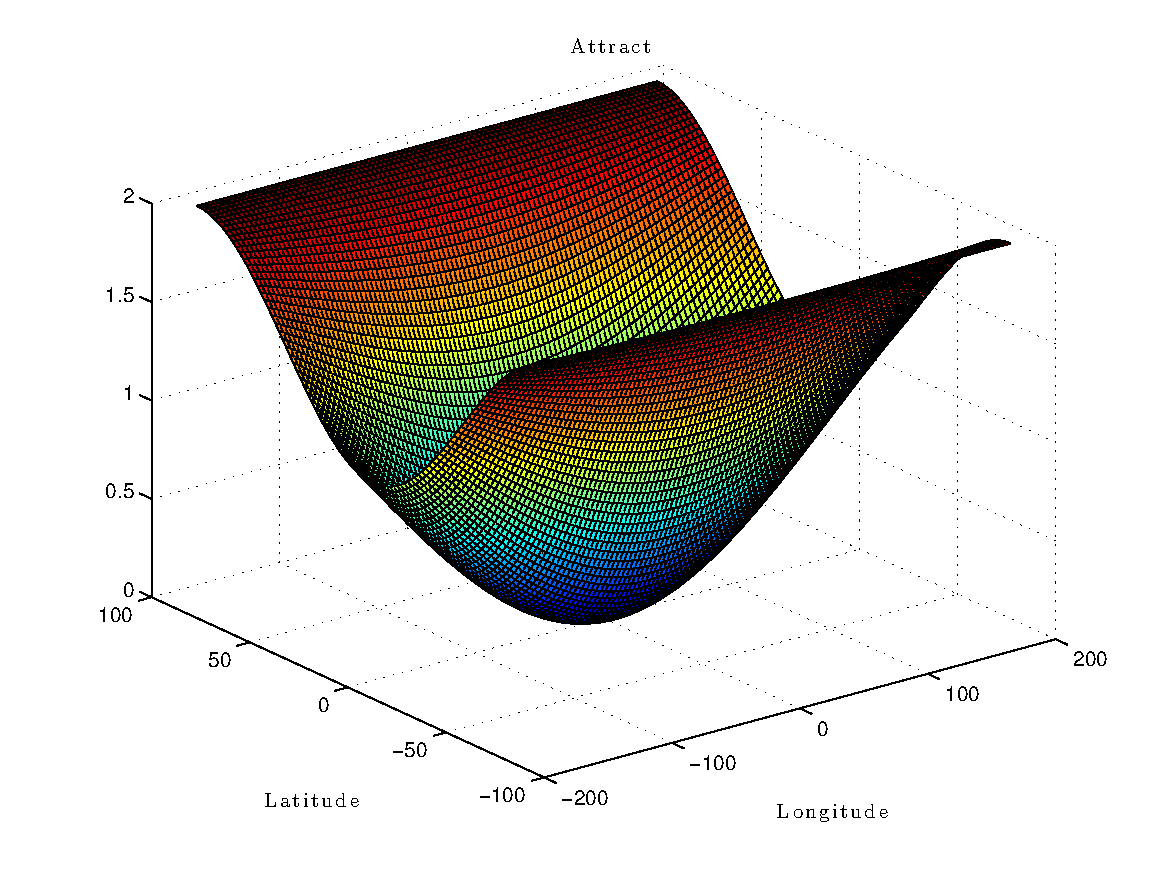
\includegraphics[width=\columnwidth]{attract_error} 
        		\caption*{Attractive \( A(R) \) } \label{fig:attract_error} 
        	\end{subfigure}~ %add desired spacing between images, e. g. ~, \quad, \qquad, \hfill etc. %(or a blank line to force the subfigure onto a new line) 
        	\begin{subfigure}[htbp]{0.3\columnwidth} 
        		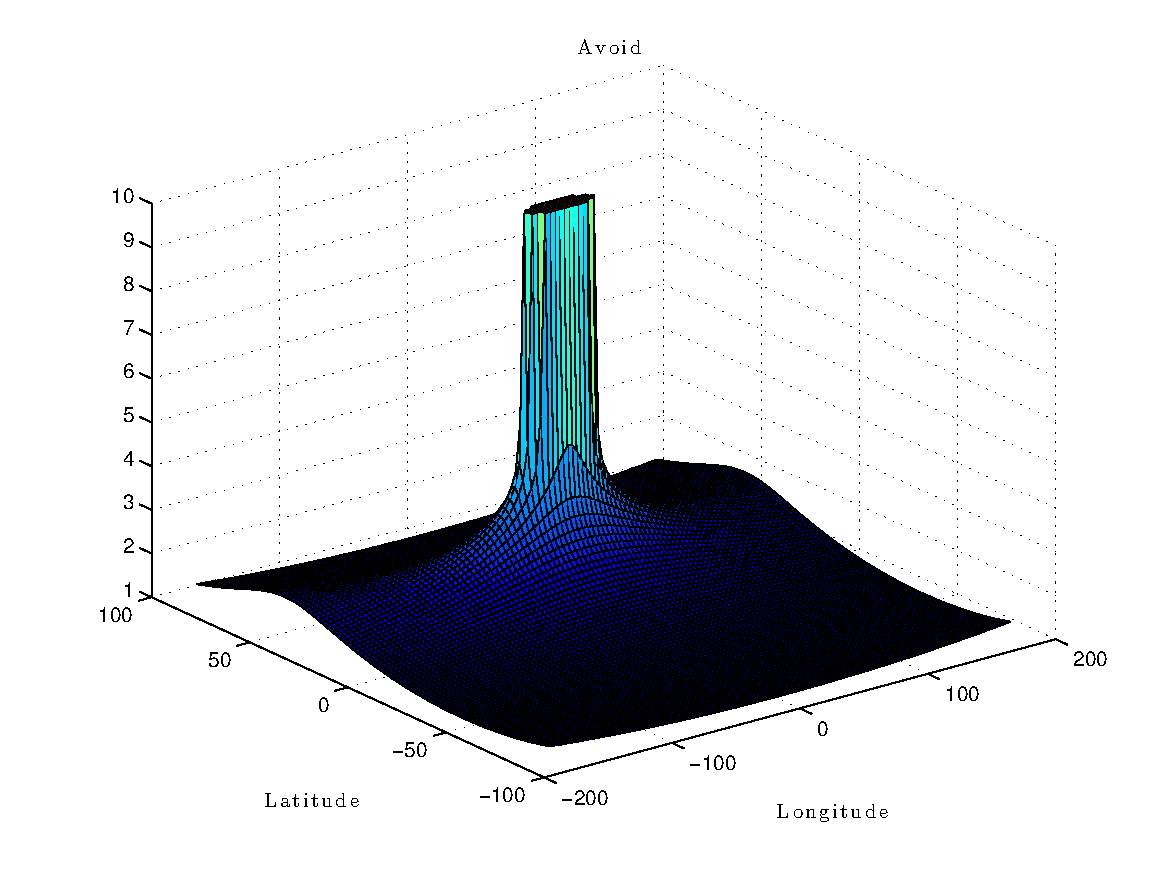
\includegraphics[width=\columnwidth]{avoid_error} 
        		\caption*{Repulsive \( B(R) \)} \label{fig:avoid_error} 
        	\end{subfigure}
        	\begin{subfigure}[htbp]{0.3\columnwidth} 
        		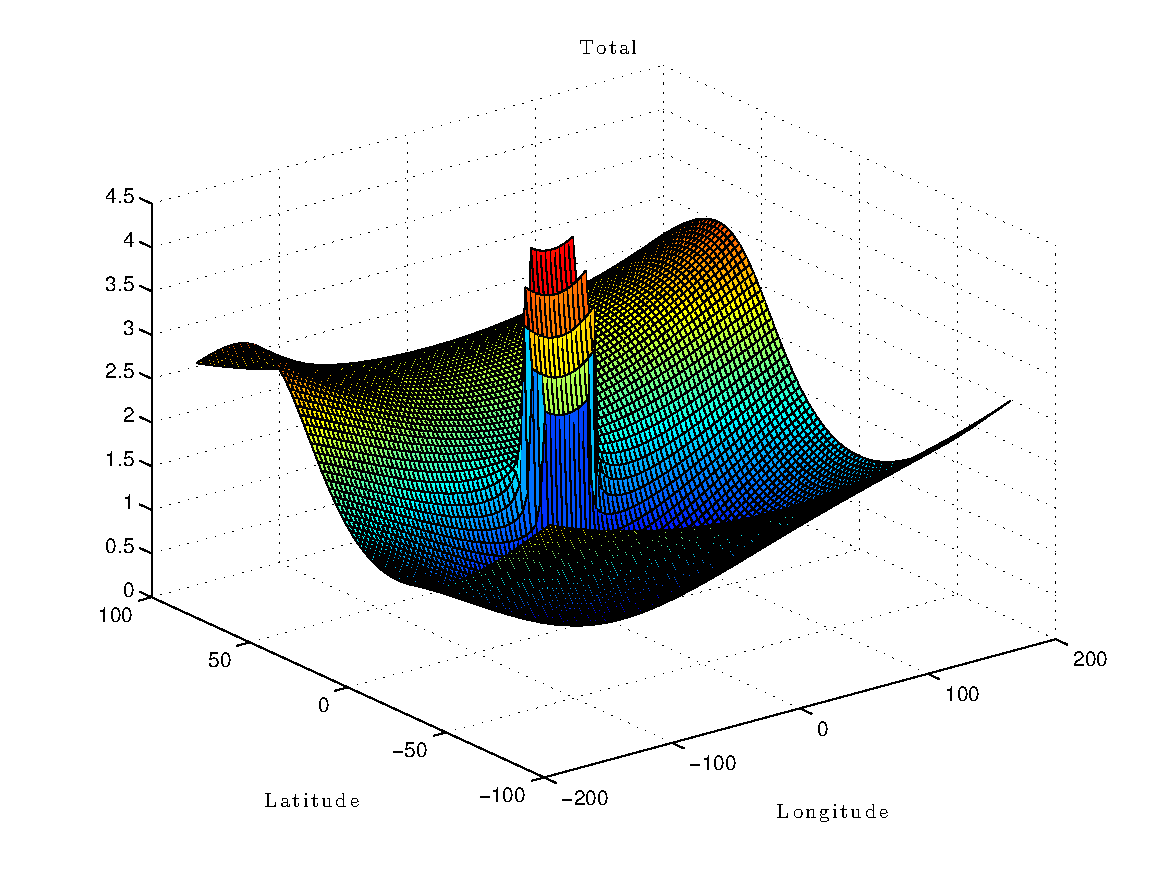
\includegraphics[width=\columnwidth]{combined_error} 
        		\caption*{Configuration \( \Psi \)} \label{fig:combined_error} 
        	\end{subfigure}
        \end{figure}
        \item We can easily generalize this technique to an arbitrary number of constraints 
			\begin{align*}
				\Psi = A \bracket{1 + \sum_i C_i} \text{ where } C_i = B - 1
			\end{align*}
		\item Lyapunov analysis is used to derive an adaptive control scheme which guarantees stability in the face of disturbances and obstacles
		\begin{align*}
			u &= - k_R e_R - k_\Omega e_\Omega + \Omega \times J \Omega - W \bar{\Delta} \\
			\dot{\bar{\Delta}} &= k_\Delta W^T \parenth{e_\Omega + c e_R} 
		\end{align*}
	\end{itemize}
\end{block} % end of structure block

\begin{block}{Numerical Simulation} % optimal control block
	\begin{itemize}
		\item \Emph{Geometric Adaptive Controller} is able to stabilize the rigid body while avoiding multiple constraints with a fixed but unknown external disturbance
		\begin{align*}
			\text{Initial: } R_0 =  \exp(\ang{225} \times \frac{\pi}{180} \hat{e}_3) \quad \text{Final: } R_d = I \quad \text{Disturbance: } \Delta = \begin{bmatrix} 0.2 & 0.2 & 0.2 \end{bmatrix}^T
		\end{align*}
		\item The adaptive controller accurately accounts for the disturbance and ensures all constraints are satisfied
	\end{itemize}
	
	\begin{figure} 
    	\centering 
    	\begin{subfigure}[htbp]{0.3\columnwidth} 
    		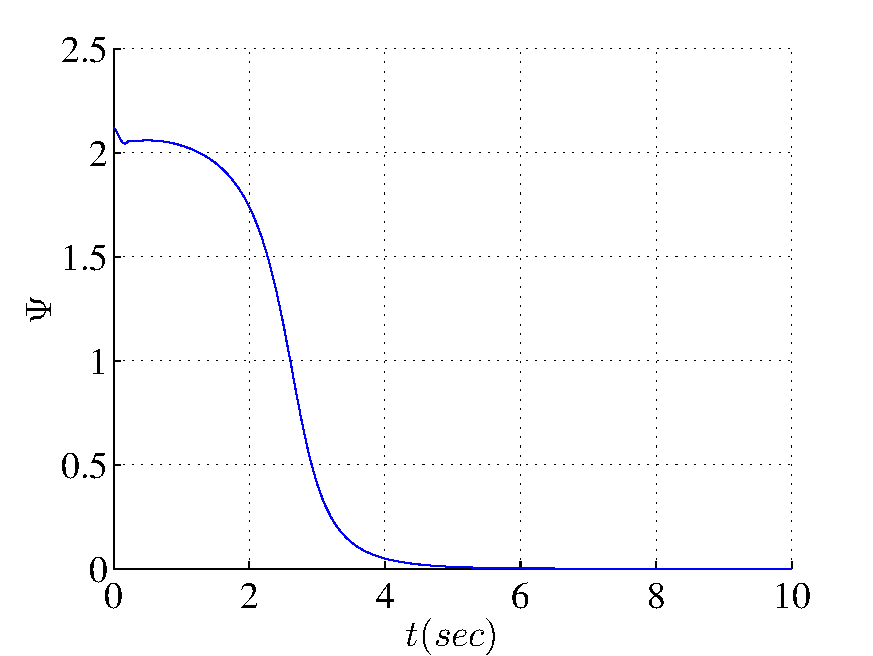
\includegraphics[height=4.15in]{Psi_adapt} 
    		\caption*{Configuration error \( \Psi \)} \label{fig:Psi_adapt} 
    	\end{subfigure}~
    	\begin{subfigure}[htbp]{0.3\columnwidth} 
    		\includegraphics[height=4.15in]{delta_adapt} 
    		\caption*{Disturbance estimate \( \bar \Delta \)} \label{fig:delta_adapt} 
    	\end{subfigure}~
    	\begin{subfigure}[htbp]{0.3\columnwidth} 
    		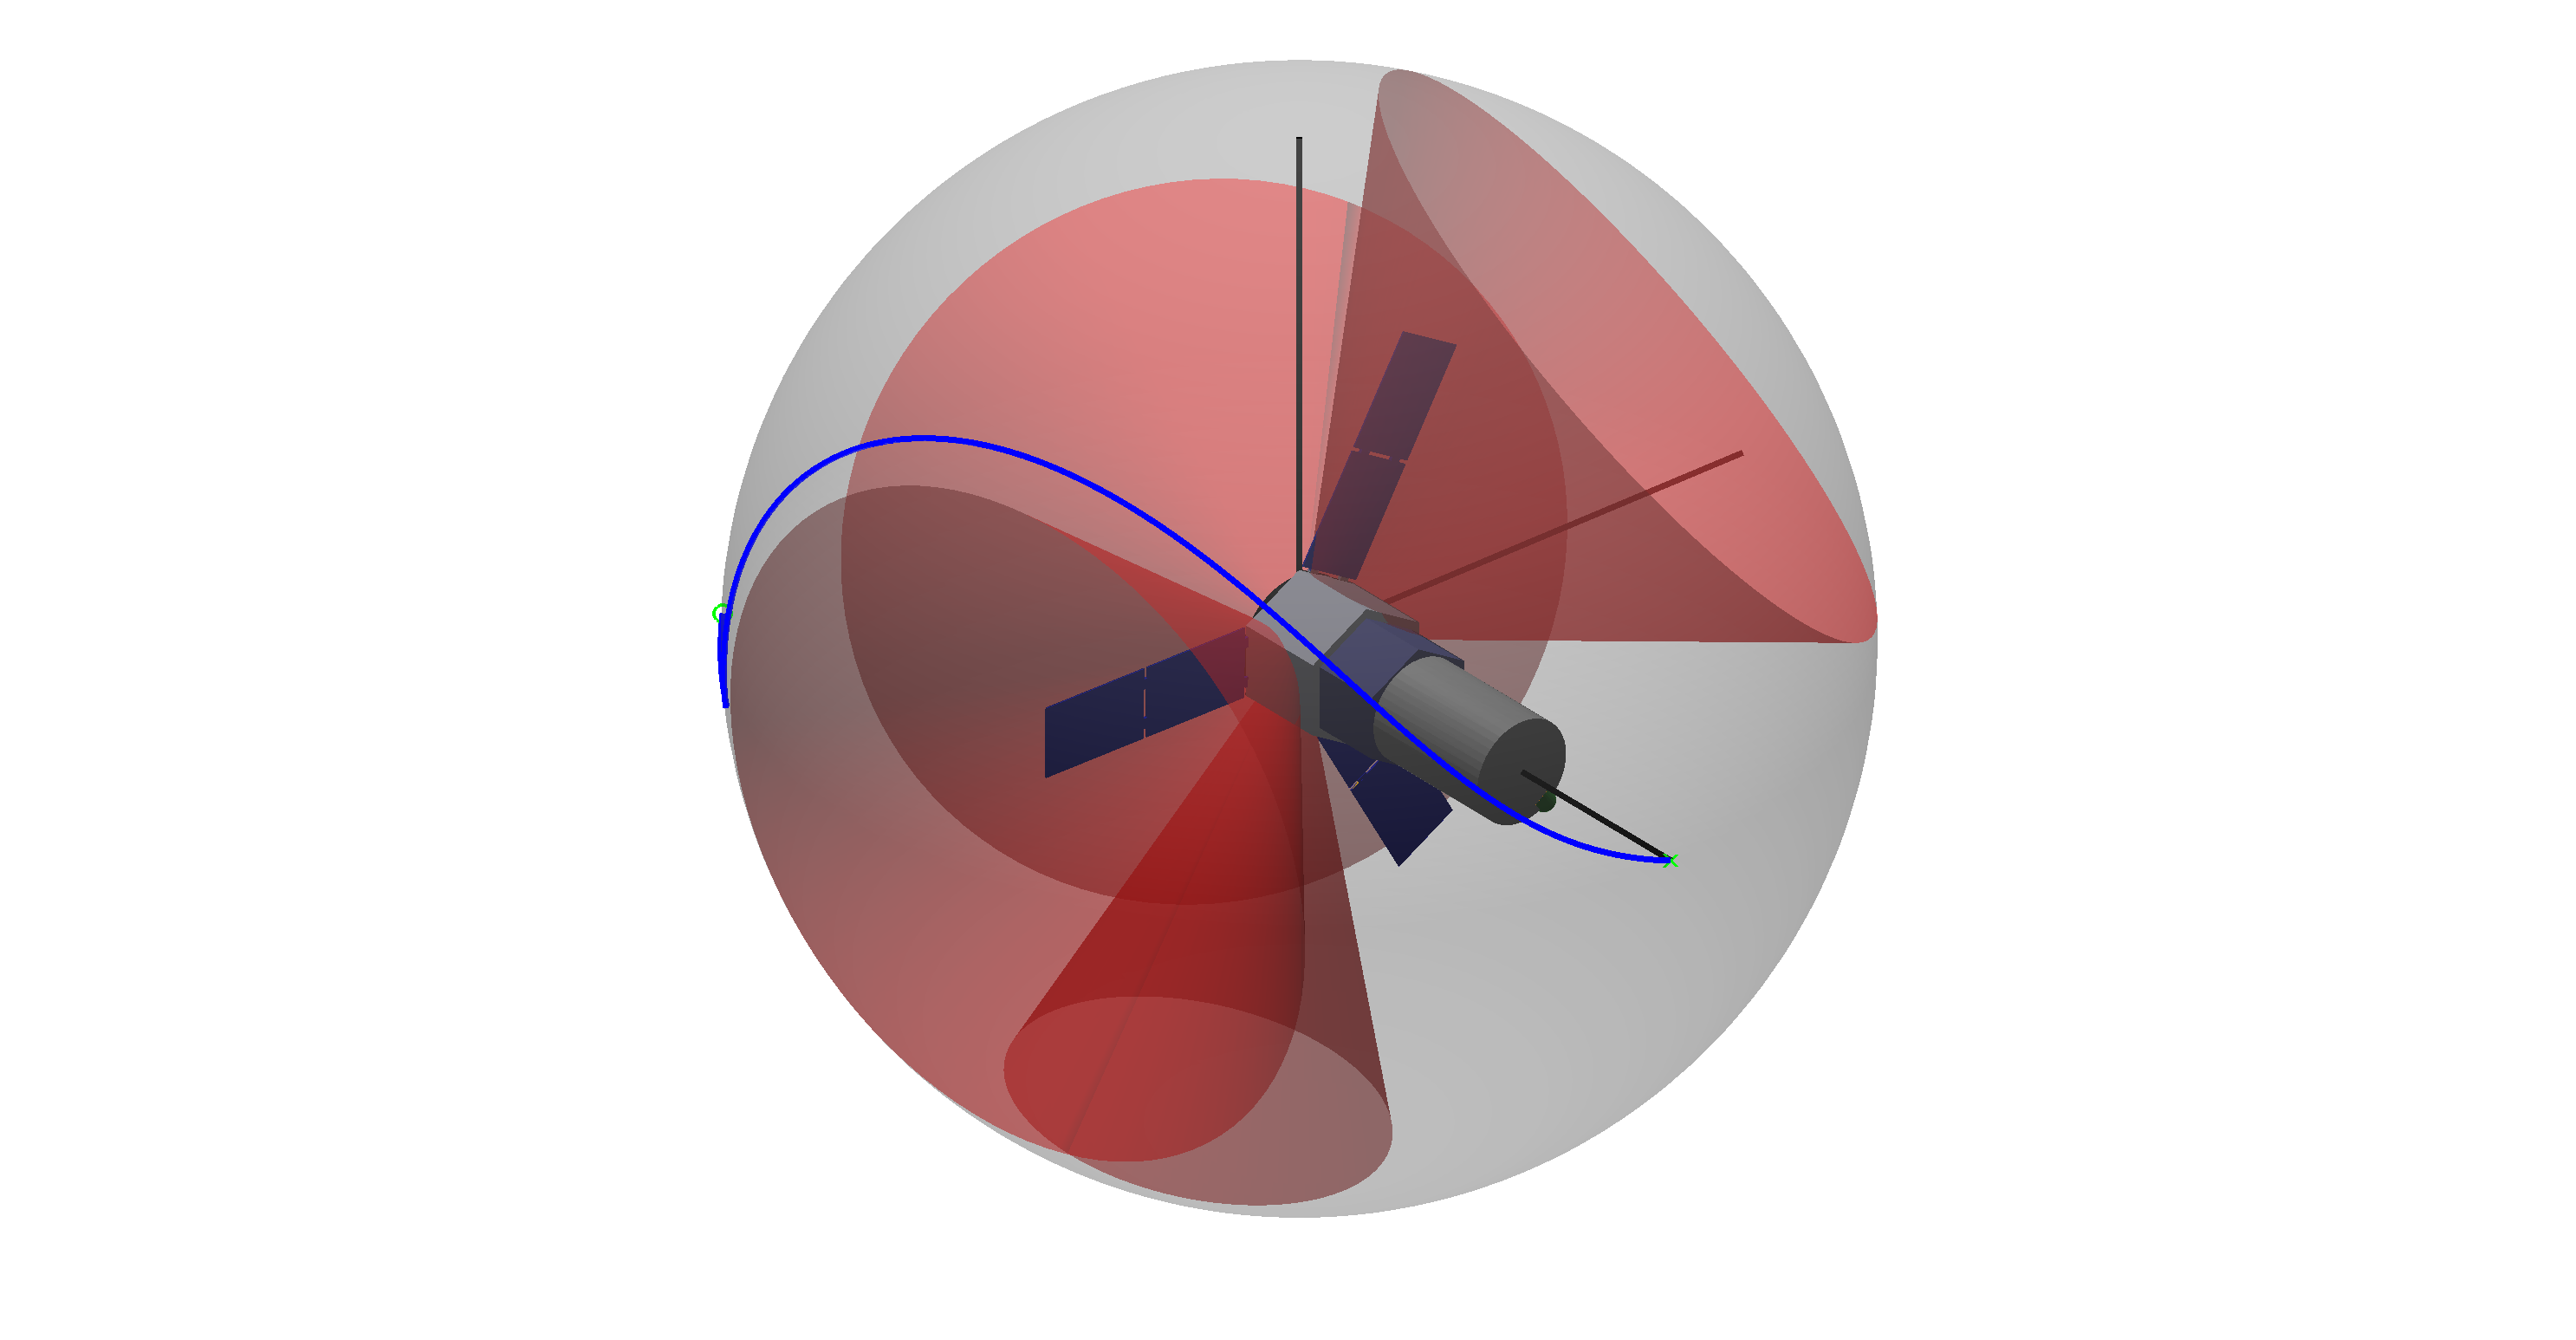
\includegraphics[trim=9cm 2.5cm 12cm 0,clip,height=4.15in]{cad_adapt} 
    		\caption*{Attitude trajectory} \label{fig:cad_adapt} 
    	\end{subfigure}
	\end{figure}
	\hfill
\end{block} % end of optimal control block
\end{column}


%-----------------------------------------------------------------------------------------
% THIRD (RIGHT) COLUMN
%---------------------------------------------------------------------------------------
\begin{column}{\onecolwidth} % third column start

\begin{block}{UAV Validation} % results block
	\begin{itemize}
		\item Hexrotor UAV developed by the \Emph{Flight Dynamics and Controls Laboratory}
		\begin{itemize}
			\item Three pairs of counter-rotating propellers
			\item Attached to a spherical joint to emulate a fully actuated rigid body
			\item Onboard computer module receives measurements from Vicon motion capture system and computes control input in real-time
		\end{itemize}
		\vspace{0.35in}
    	\begin{figure}
    		\centering
    		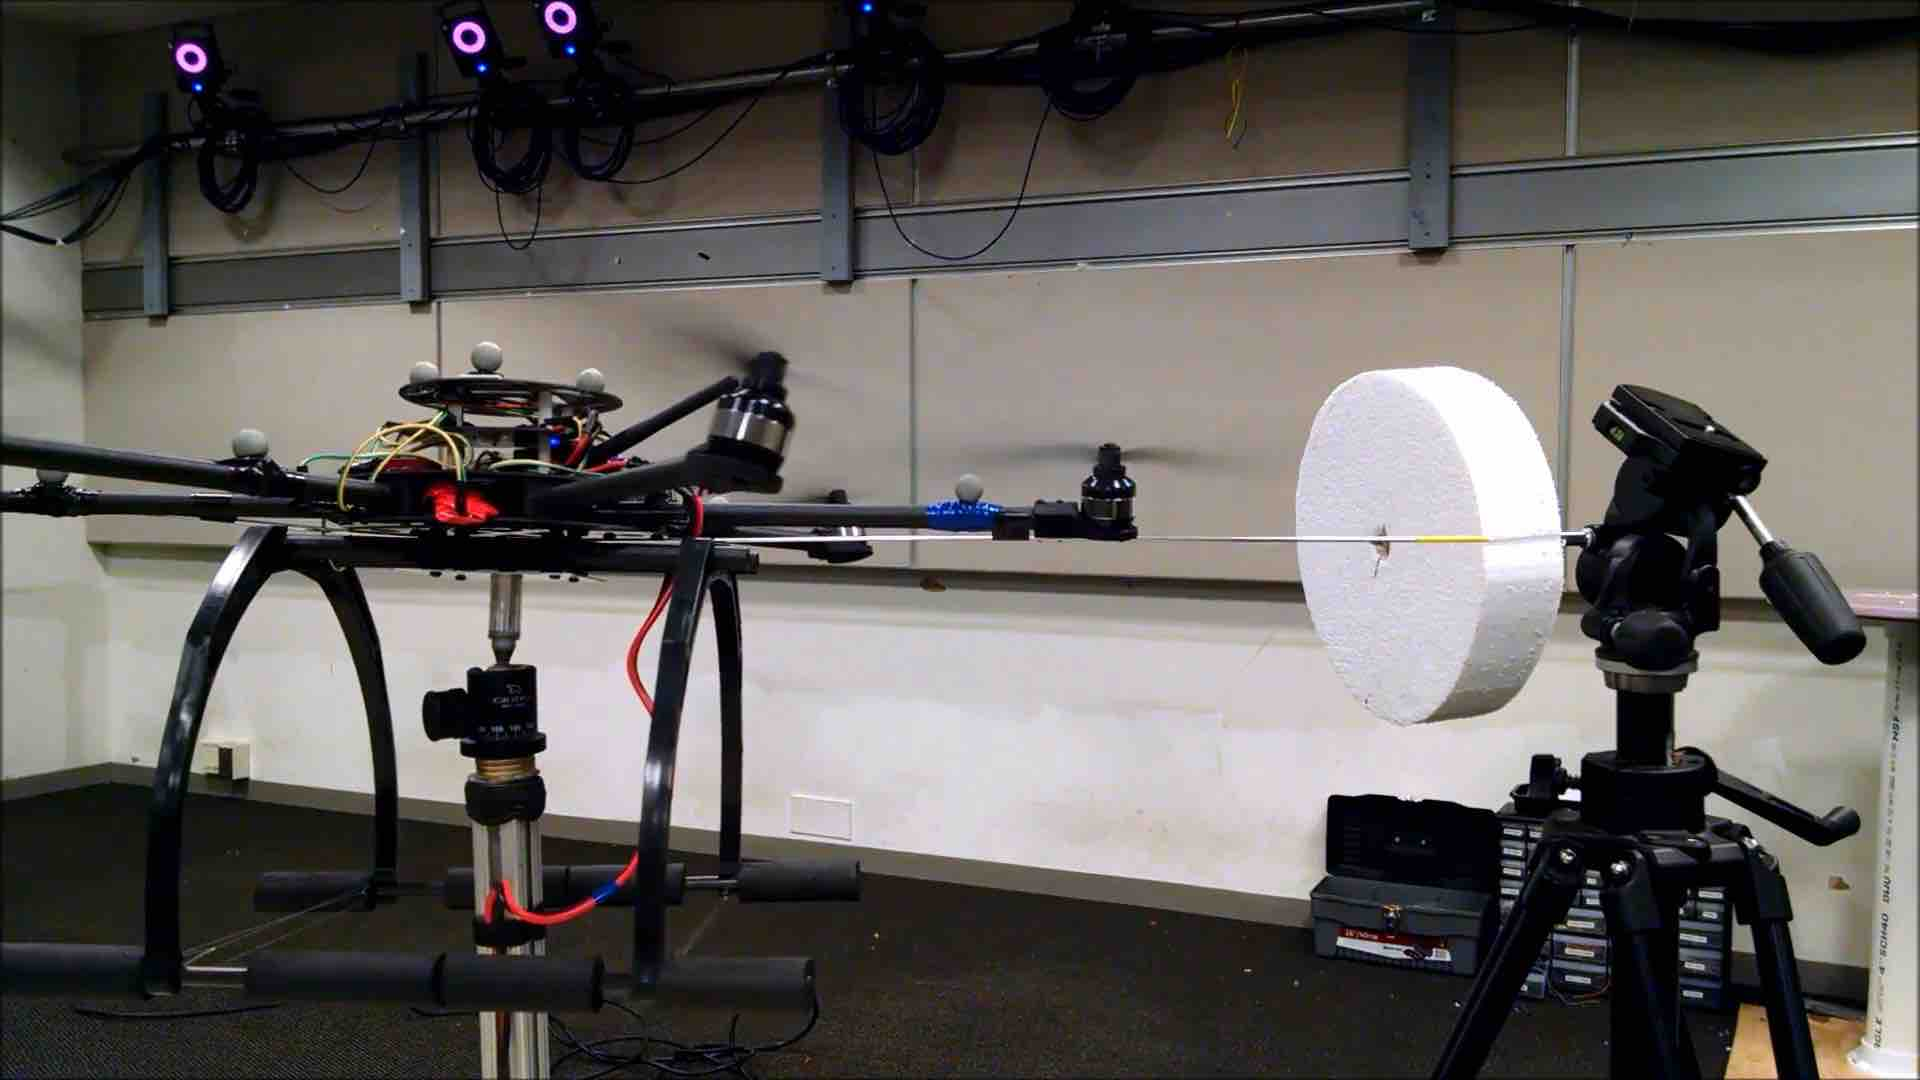
\includegraphics[width = 0.7\columnwidth]{hexrotor}
    		\caption*{Attitude control testbed~\label{fig:hexrotor}}
    	\end{figure}
		\item Hexrotor rotates about vertical axis while automatically avoiding the obstacle
		\begin{align*}
			\text{Initial: } R_0 = \exp( \frac{\pi}{2} \hat{e}_3) \quad \text{Final: } R_d = I
		\end{align*}
	\end{itemize}
	\begin{figure} 
	\centering 
	\begin{subfigure}[htbp]{0.5\columnwidth} 
		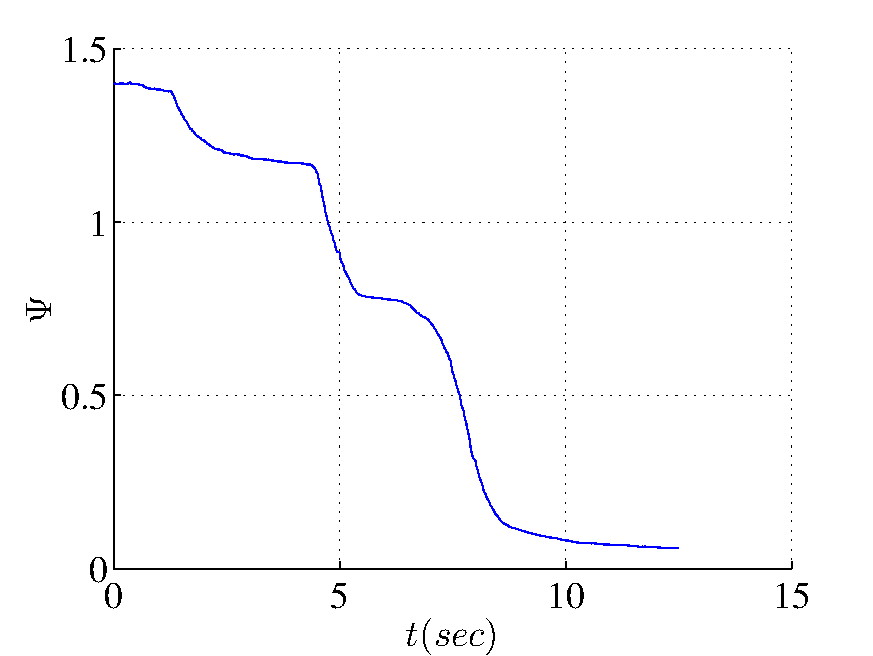
\includegraphics[width=\columnwidth]{Psi_exp} 
		\caption*{Configuration error \( \Psi \)} \label{fig:Psi_exp} 
	\end{subfigure}~
	\begin{subfigure}[htbp]{0.5\columnwidth} 
		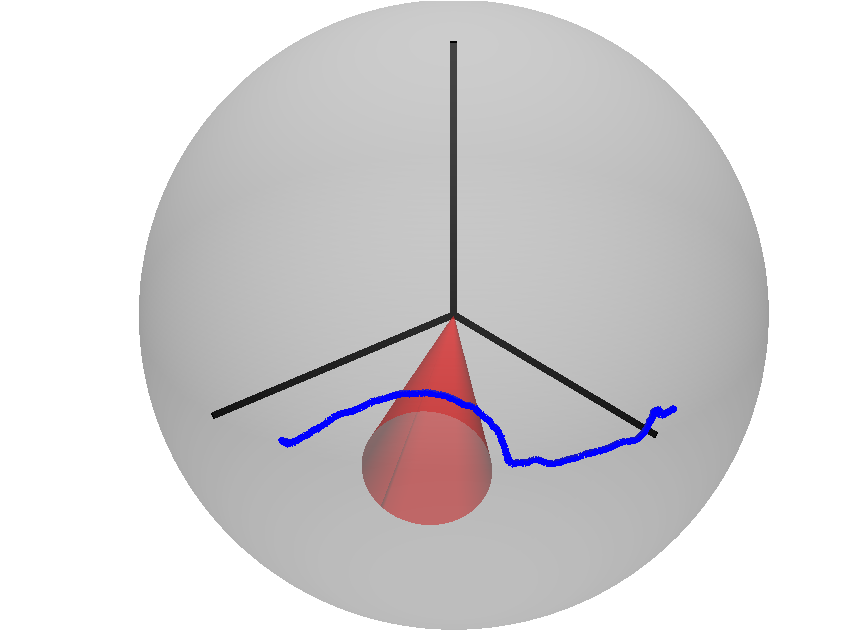
\includegraphics[width=\columnwidth]{traj_exp} 
		\caption*{Attitude Trajectory} \label{fig:traj_exp} 
	\end{subfigure}
	\end{figure}
	\begin{itemize}
		\item Adaptive controller is robust to uncertainties and disturbances 
	\end{itemize}
\end{block} % end of results block

\begin{block}{Conclusions} % conclusion
	\begin{itemize}
		\item Constrained geometric adaptive controller on \( \SO \)
		\begin{itemize}
			\item Completely avoids singularities and ambiguities 
			\item Geometrically exact and conceptually simple attitude controller
			\item Automatically satisfies multiple constraints without added complexity
		\end{itemize}
		\item Obstacle avoidance computed in real-time with on-board software
		\begin{itemize}
			\item Typical planning methods are only able to determine an obstacle-free path after multiple iterations and extensive computation
			\item Large computation costs limit these methods to a priori calculation and make responsive control impossible
			\item Randomized search algorithms can only offer a stochastic guarantee of convergence as the computation time increases
		\end{itemize}
		\item Our control system is capable of handling any number of obstacles and offers a rigorous stability proof
		\begin{itemize}
			\item Ideal for challenging scenarios with multiple obstacles or an environment which requires complex control
			\item Computationally efficient and ideal for embedded systems with energy or computation limitations
			\item Stability proof ensures manuvers always satisfy pointing constraints 
		\end{itemize}
	\end{itemize}
\end{block} % conclusion
\end{column}  % third column end

\end{columns} % end of all columns in poster
\end{frame} % end of enclosing frame
\end{document}